\documentclass{article}
\usepackage[utf8]{inputenc}
\usepackage{kotex}
\usepackage{verbatim}
\usepackage{graphicx}
\usepackage{indentfirst}
\usepackage{subfigure}
\usepackage{listings}
\usepackage{xcolor}
\usepackage{cprotect}
\usepackage{tikz}
\usetikzlibrary{graphdrawing.trees}
\usepackage{geometry}
\usepackage{environ}
\usepackage{amsmath}
\usepackage{amssymb}
\usepackage{enumitem}
\usepackage{verbatim}

\renewcommand{\figurename}{그림}
\renewcommand{\tablename}{표}
\renewcommand{\contentsname}{목차}
\renewcommand{\lstlistingname}{코드}
\renewcommand{\listfigurename}{\figurename 목차}
\renewcommand{\listtablename}{\tablename 목차}
\renewcommand{\lstlistlistingname}{\lstlistingname 목차}

\geometry{
    a4paper,
    left=30mm,
    right=30mm,
    top=30mm,
    bottom=40mm
}

\lstset{language=C++,
            basicstyle=\ttfamily,
            keywordstyle=\color{blue}\ttfamily,
            stringstyle=\color{red}\ttfamily,
            commentstyle=\color{teal}\ttfamily,
            numberstyle=\tiny\color{gray}\ttfamily,
            morecomment=[l][\color{magenta}]{\#}
            breakatwhitespace=false,         
            breaklines=true,                 
            captionpos=b,                    
            keepspaces=true,                 
            numbers=left,                    
            numbersep=5pt,                  
            showspaces=false,                
            showstringspaces=false,
            showtabs=false,                  
            tabsize=2
}

\title{자료구조 HW12 AVL tree}
\author{C211123 이준선}
\date{2022년 12월 16일}

\begin{document}

\maketitle
\tableofcontents
\listoffigures
\lstlistoflistings

\maketitle

\section{개요}
AVL tree를 구현하였고, AVL tree의 핵심인 LL, LR, RR, RL 회전에 대한 설명을 담았다. 또한 클래스 구현 내용과 설계 내용을 담았다.

\textbf{Note :} \LaTeX 보고서의 tex 파일엔 tikz package의 graphdrawing.tree library가 담겼습니다. 이 라이브러리는 \textbf{`Lua\LaTeX'} 컴파일러 환경에서만 작동하므로, 확인 시 Lua\LaTeX 컴파일러로 실행해주십시오. 일반적으로 많이 쓰이는 pdf\LaTeX에서는 컴파일되지 않습니다.

\section{Class 설계 내용 및 이유}
\begin{lstlisting} [language=C++, escapeinside=``, caption=AVL.h, label={lstlisting:AVL.h}]
#ifndef AVL_H
#define AVL_H
#include <queue>
#include <iostream>
using namespace std;

class Node {
public:
	int GetBF();
	int GetData();
	void SetData(const int data);
	void SetBF(const int bf);
	Node* GetLeftChild();
	Node* GetRightChild();
	Node* GetParent();
	void SetLeftChild(Node* leftChild);
	void SetRightChild(Node* rightChild);
	void SetParent(Node* parent);
	Node(int data, int bf, Node* leftChild, Node* rightChild, Node* parent);
	Node(int data);
	Node();

	Node*& GetLeftChildRef();
	Node*& GetRightChildRef();
	Node*& GetParentRef();
private:
	int data;
	int bf;
	Node* leftChild;
	Node* rightChild;
	Node* parent;
};

class bstree {
private:
	bool rotation(Node* start, Node* end);
	inline void changeLeftSubtree(Node* main, Node* sub);
	inline void changeRightSubtree(Node* main, Node* sub);
	int GetHeight(Node* root);
	int GetBalanceFactor(Node* root);
	Node* rotateLL(Node* root);
	Node* rotateRR(Node* root);
	Node* rotateLR(Node* root);
	Node* rotateRL(Node* root);
	void Rebalance(Node*& root);
	Node* findMin(Node* root);
	Node* findNode(const int key, Node* root);
	Node* InorderSucc(Node* current);
	void ResetParent(Node*& root);
	void ResetBF(Node*& root);
	void remove(const int key, Node*& root);
public:
	void visit(Node* ptr);
	void insert(const int value, Node*& root);
	void Showresult(Node* root);
	bool Search(const int key, Node* root);
	void del(const int key, Node*& root);
	void clear(Node*& root);
};
#endif
\end{lstlisting}

코드 \ref{lstlisting:AVL.h}에 클래스 설계 내용을 담은 헤더 파일이 나와 있다. 명세서에서는 Node를 struct로 정의했지만 여기서는 클래스로 정의하는 것이 더 편하기에 클래스로 바꾸었다. 객체 지향 설계 원칙에 맞추어 내부 함수와 내부 변수는 최대한 정보를 감추고, 필요한 경우에만 외부 함수를 통해서 접근하도록 설계하였다. 먼저 Node 클래스의 경우, 데이터를 담는 int형 data, 그리고 balance factor를 의미하는 bf, 왼쪽 서브 트리, 오른쪽 서브 트리, 그리고 부모 서브 트리를 각각 의미하는 leftChild, rightChild, parent가 private 멤버로 존재한다. Node 클래스는 public 함수로 각각의 get, set 함수를 제공하여 이에 접근할 수 있도록 한다. 한편 특별히 leftChild, rightChild, parent에는 get, set 함수 이외에도 getref 함수가 존재한다. 이는 getref 함수를 통해서 private 변수에 직접 접근할 수 있으므로 객체 지향 설계에 위배될 수 있으나, bstree에서는 계속적으로 재귀 함수를 통해 구현을 이어가기에 편의성을 위해 만들었다. 따라서 getref 함수는 변수에 직접 접근할 수 있으므로 주의해서 사용하되 재귀적 구현에서 매우 유용한 도구가 된다\footnote{정확히 말하면 재귀적 구현에서 인자로 Node*\& 형식의 참조를 매개 인자로 받을 때 사용되며, private한 변수에 직접 접근하여 수정할 수 있도록 하려면 getref 함수가 필수적으로 필요하다.}. parent는 노드 자체가 부모의 정보 역시 포함하도록 설계하였다. 이 경우 삽입, 삭제, 회전 등의 연산에서 매번 parent의 정보를 관리해주는 단점이 있으나, 그에 대응하는 여러 가지 장점들이 있다. 부모 정보를 포함하므로 InorderSuccessor() 함수 구현하기가 쉬워지며, 매번 parent 정보를 찾기 위해 root 노드를 가지고 다니며 새롭게 계산해줄 필요가 없어서 성능 개선의 여지가 있다.

bstree 노드의 경우 트리를 구성하는데 필요한 기능들을 담고 있다. 사용자에게 공개된 함수는 visit, insert, showresult, Search, del, clear\footnote{트리 내 모든 데이터를 지우는 함수, 과제 자체에는 필요 없는 내부적 테스트를 위한 함수이나 vector 클래스의 clear 함수처럼, 사용자에게 public하게 공개되기에 적절한 함수이며 테스트 과정 또한 과제의 일부라 판단되어 남겨두었다. 메뉴 선택 시 5번을 선택하면 clear 함수를 이용할 수 있다.} 함수 뿐이며, 나머지 함수들은 내부적 구현을 위해 private하게 숨겨져 있다.

Node 내부 변수인 data, bf, 그리고 자식과 부모 노드의 경우 Node 클래스에서 자체적으로 이에 접근 및 수정하도록 함수를 구성하였고, bstree는 Node의 변수에는 직접적으로 접근하지는 않지만 Node를 이용해서 AVL tree를 구성하는데 필요한 모든 연산을 처리한다. 다른 방법으로는 Node를 bstree의 friend 클래스로 선언해서, bstree에서 Node의 모든 private 변수에 직접적으로 접근이 가능하게끔 구현하는 방법도 있다. Node가 현재로썬 확실하게 bstree에 귀속되는 클래스이기에 가능한 방법이다.

\section{결과}
\begin{figure}
    \centering
    \subfigure[Initial result]{
        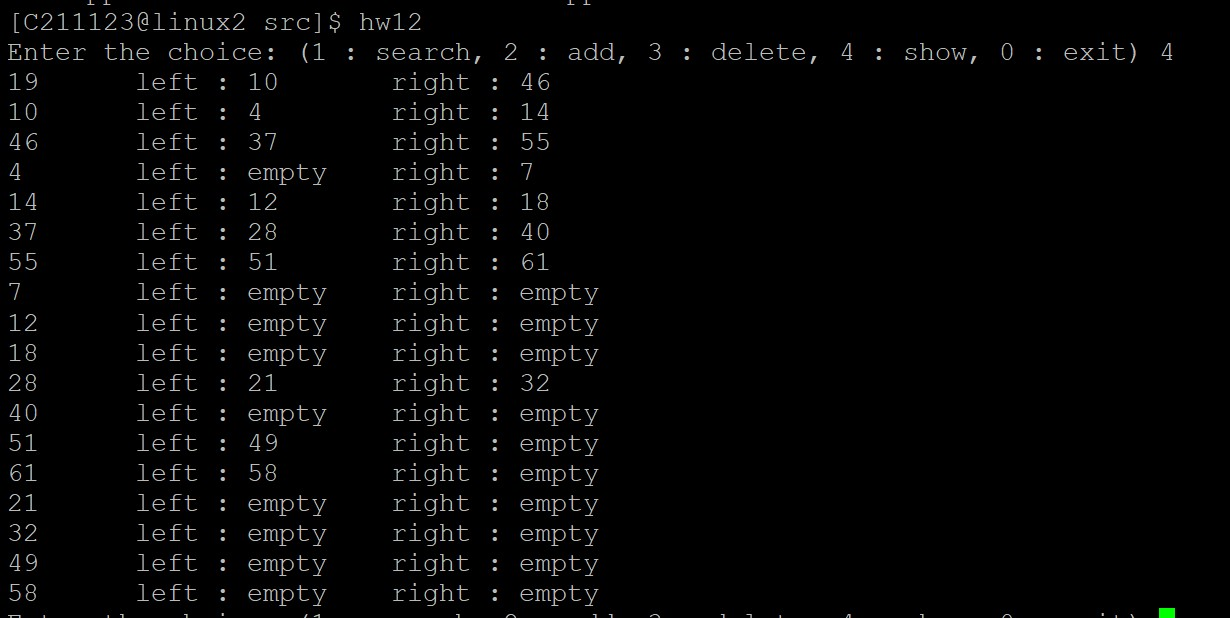
\includegraphics[width=0.64\textwidth]{result_initial_show.jpg}
        \label{fig:initial result console}
    }
    \subfigure[initial result tree]{
    \resizebox{0.64\textwidth}{!}{ %
        \begin{tikzpicture} [nodes={draw, circle}]
        \node{19}
        child { node {10}
            child { node {4}
                child [missing]
                child { node {7} }
            }
            child [missing]
            child { node {14} 
                child { node{12} }
                child { node{18} }
            }
        }
        child [missing]
        child [missing]
        child [missing]
        child [missing]
        child { node{46}
            child { node {37}
                child { node{28}
                    child { node{21} }
                    child { node{32} }
                }
                child { node {40} }
            }
            child[missing]
            child { node {55} 
                child { node {51} 
                    child { node {49} }
                    child [missing]
                }
                child { node{61} 
                    child { node {58} }
                    child [missing]
                }
            }
        };
        \end{tikzpicture}
        } %
        \label{fig:initial result tree}
    }
    \caption{Initial Result}
    \label{fig:Initial Result}
\end{figure}

그림 \ref{fig:Initial Result}는 명세서에서 주어진 초기 Insert input값에 대한 AVL tree이며, \ref{fig:initial result tree}는 \ref{fig:initial result console}의 출력 결과를 트리로 표현한 것이다. \ref{fig:initial result tree}에서 모든 서브트리의 BF가 2 미만으로 잘 균형이 맞아 떨어진 것을 확인할 수 있다.

\begin{figure}
    \centering
    \subfigure[Result of searching 18]{
        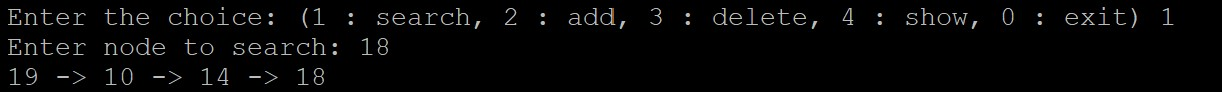
\includegraphics[width=0.64\textwidth]{find_18.jpg}
        \label{fig:seach 18 console result}
    }
    \subfigure[Path to 18]{
        \resizebox{0.64\textwidth}{!}{ %
        \begin{tikzpicture} [nodes={draw, circle}]
        \node[fill=orange]{\textbf{19}}
        child { node[fill=orange] {\textbf{10}}
            child { node {4}
                child [missing]
                child { node {7} }
            }
            child [missing]
            child { node[fill=orange] {\textbf{14}} 
                child { node{12} }
                child { node[fill=orange]{\textbf{18}} }
            }
        }
        child [missing]
        child [missing]
        child [missing]
        child [missing]
        child { node{46}
            child { node {37}
                child { node{28}
                    child { node{21} }
                    child { node{32} }
                }
                child { node {40} }
            }
            child[missing]
            child { node {55} 
                child { node {51} 
                    child { node {49} }
                    child [missing]
                }
                child { node{61} 
                    child { node {58} }
                    child [missing]
                }
            }
        };
        \end{tikzpicture}
        } %
        \label{fig:path to 18 tree}
    }
    \caption{Search : 18}
    \label{fig:search 18}
\end{figure}

그림 \ref{fig:search 18}에서 18을 검색하는 모습을 볼 수 있으며, 18까지의 경로인 19$\rightarrow$10$\rightarrow$14$\rightarrow$18가 잘 출력된 것을 그림 \ref{fig:seach 18 console result}에서 확인할 수 있다. 그림 \ref{fig:path to 18 tree}은 그림 \ref{fig:seach 18 console result}의 출력 결과를 tree에 시각화한 것이다.

\begin{figure}
    \centering
    \subfigure[Result of insert 9]{
        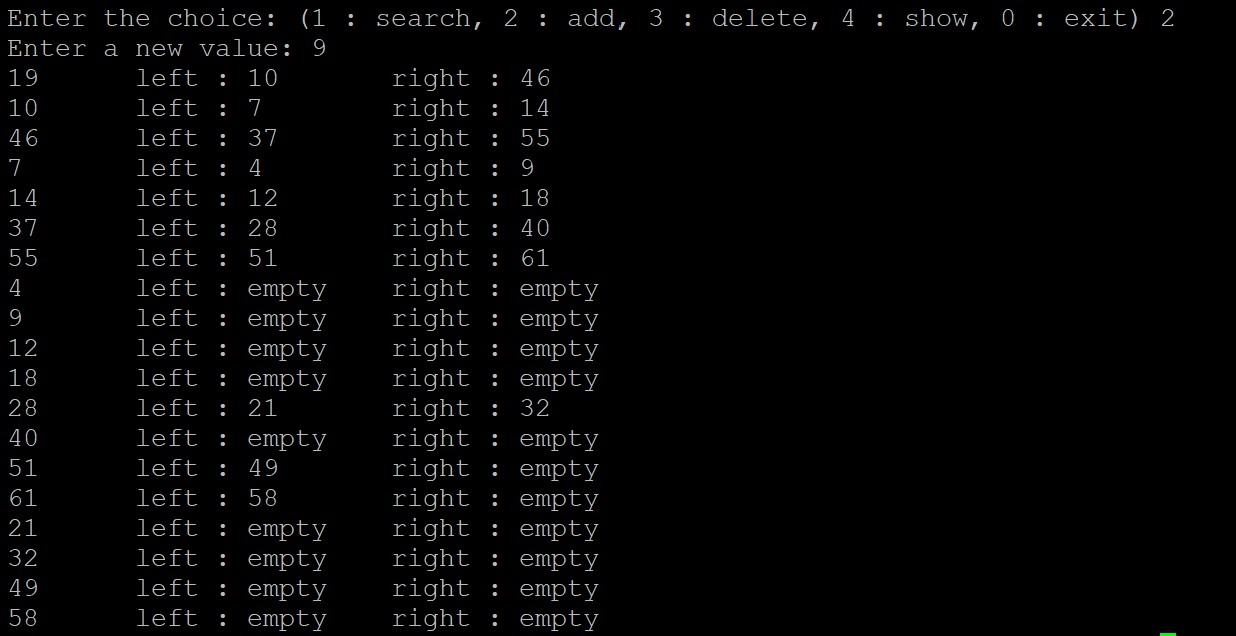
\includegraphics[width=0.64\textwidth]{result_insert_9.jpg}
        \label{fig:result insert 9 console}
    }
    \subfigure[Result of insert 9 tree]{
        \resizebox{0.64\textwidth}{!}{ %
        \begin{tikzpicture} [nodes={draw, circle}]
        \node{19}
        child { node {10}
            child { node {7}
                child { node {4} }
                child { node {9} }
            }
            child [missing]
            child { node {14} 
                child { node{12} }
                child { node{18} }
            }
        }
        child [missing]
        child [missing]
        child [missing]
        child [missing]
        child { node{46}
            child { node {37}
                child { node{28}
                    child { node{21} }
                    child { node{32} }
                }
                child { node {40} }
            }
            child[missing]
            child { node {55} 
                child { node {51} 
                    child { node {49} }
                    child [missing]
                }
                child { node{61} 
                    child { node {58} }
                    child [missing]
                }
            }
        };
        \end{tikzpicture}
        } %
        \label{fig:result insert 9 tree}
    }
    \caption{After insert 9}
    \label{fig:result insert 9}
\end{figure}

그림 \ref{fig:result insert 9}에서 9를 삽입했을 때의 결과를 볼 수 있다. 그림 \ref{fig:result insert 9 tree}에서 그림 \ref{fig:result insert 9 console}의 출력 결과를 시각화한 것을 볼 수 있다. 일반 이진 검색 트리(Binary Search Tree, 이하 BST)에서는 9는 노드 7의 RightChild로 삽입됐을 것이지만, AVL tree에서는 4의 BF가 2가 되어 균형이 깨지므로, LR 회전하여 균형을 적절하게 이뤘음을 알 수 있다.

\begin{figure}
    \centering
    \subfigure[Result of remove 19]{
        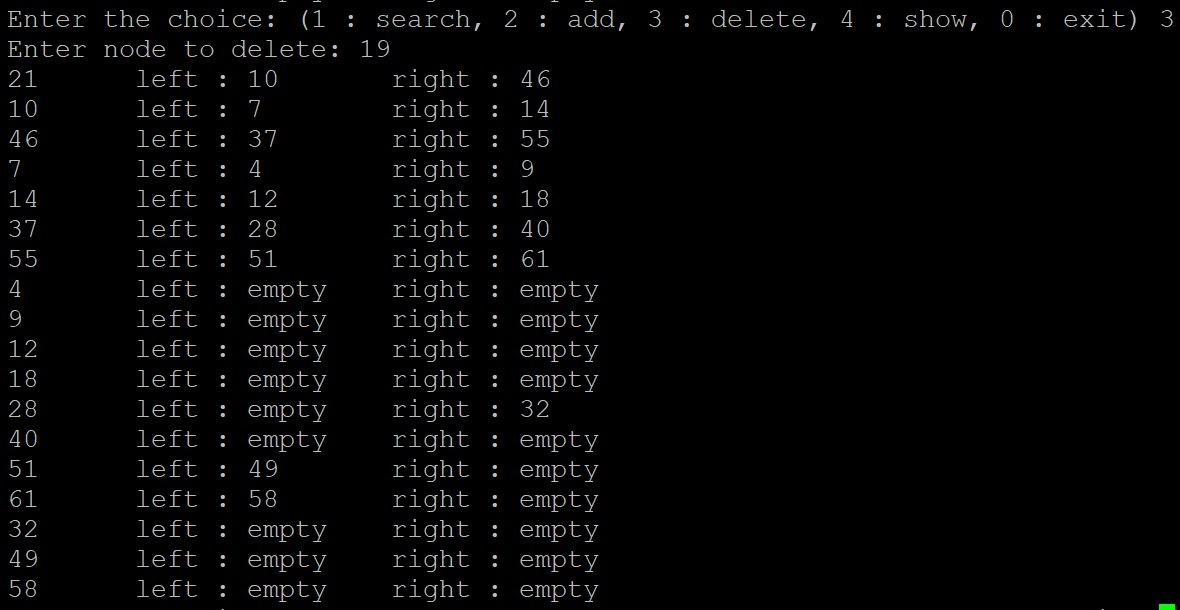
\includegraphics[width=0.64\textwidth]{remove_19.jpg}
        \label{fig:result remove 19 console}
    }
    \subfigure[Result of remove 19 tree]{
    \resizebox{0.64\textwidth}{!}{ %
        \begin{tikzpicture} [nodes={draw, circle}]
        \node{21}
        child { node {10}
            child { node {7}
                child { node {4} }
                child { node {9} }
            }
            child [missing]
            child { node {14} 
                child { node{12} }
                child { node{18} }
            }
        }
        child [missing]
        child [missing]
        child [missing]
        child [missing]
        child { node{46}
            child { node {37}
                child { node{28}
                    child [missing]
                    child { node{32} }
                }
                child { node {40} }
            }
            child[missing]
            child { node {55} 
                child { node {51} 
                    child { node {49} }
                    child [missing]
                }
                child { node{61} 
                    child { node {58} }
                    child [missing]
                }
            }
        };
        \end{tikzpicture}
        } %
        \label{fig:result remove 19 tree}
    }
    \caption{After remove 19}
    \label{fig:result remove 19}
\end{figure}

그림 \ref{fig:result remove 19}에서 19를 삭제했을 때 결과를 확인할 수 있다. 그림 \ref{fig:result remove 19 tree}에서 19의 Successor인 21이 19와 자리를 교환한 것을 알 수 있다.

\begin{figure}
    \centering
    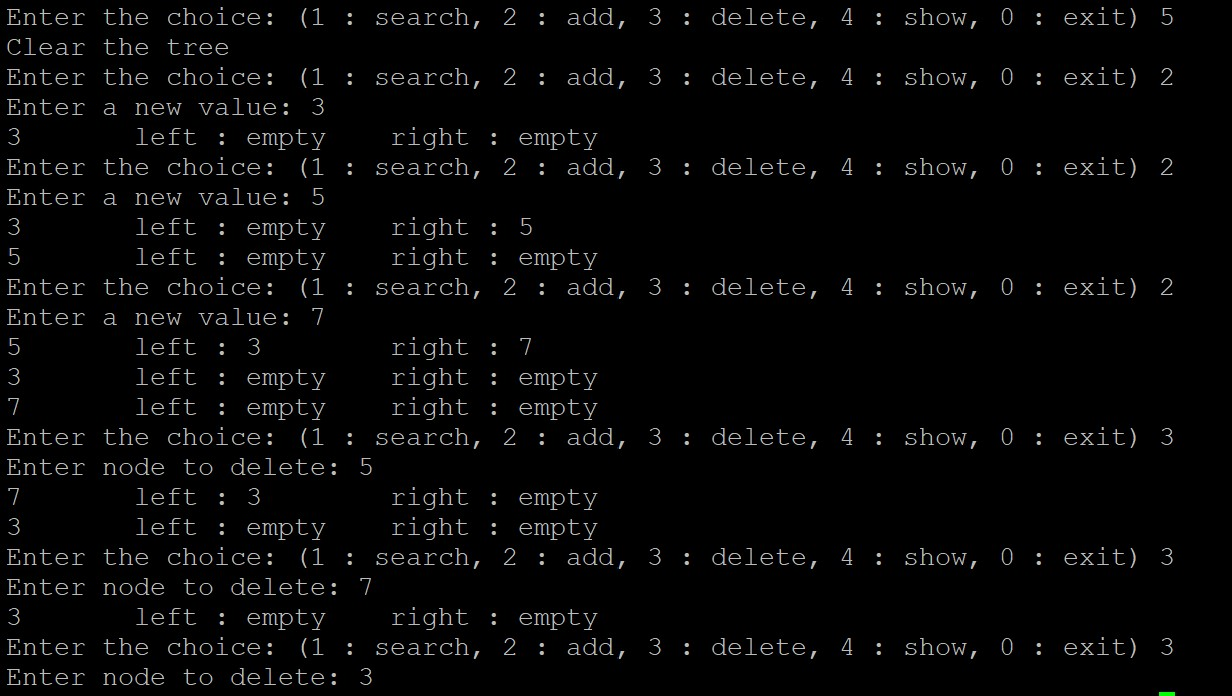
\includegraphics[width=0.64\textwidth]{insert_and_remove_357.jpg}
    \caption{빈 트리에서 3, 5, 7의 삽입과 삭제}
    \label{fig:insert and remove 357}
\end{figure}

그림 \ref{fig:insert and remove 357}에서 빈 트리에서의 삽입과 삭제 과정이 정상적으로 이루어지고 있음을 확인할 수 있다. 5번은 모든 트리를 비우는 Clear 기능이다. 이 이후에 순서대로 3, 5, 7의 삽입이 이루어지고, 5, 7, 3의 순서대로 삭제가 이루어진다. 3, 5, 7의 삽입 과정에서 RR 회전이 이루어졌음을 확인할 수 있다. 삭제 과정에서도 정상적으로 모든 노드를 삭제하였고, root 노드가 빈 상태에서도 정상적으로 프로그램이 작동함을 알 수 있다. root 노드가 빈 상태에서도 새롭게 insert하면 정상적으로 작동한다.

\section{AVL tree에서의 회전}
AVL tree의 핵심은 회전이다. AVL tree에서는 삽입된 노드와 밸런스가 꺠진 노드 사이의 위치 관계를 기준으로 다음 4가지 상황을 정의하고 있다.
\begin{itemize}
    \item LL : 임의의 노드 A를 기준으로 왼쪽 Subtree의 왼쪽 서브트리에 의해 A의 균형 인수 BF가 +2 이상으로 균형이 깨진 경우
    \item RR : 임의의 노드 A를 기준으로 오른쪽 Subtree의 오른쪽 서브트리에 의해 A의 균형 인수 BF가 -2 이하로 균형이 깨진 경우
    \item LR : 임의의 노드 A를 기준으로 왼쪽 Subtree의 오른쪽 서브트리에 의해 A의 균형 인수 BF가 +2 이상으로 균형이 깨진 경우
    \item RL : 임의의 노드 A를 기준으로 오른쪽 Subtree의 왼쪽 서브트리에 의해 A의 균형 인수 BF가 -2 이하로 균형이 깨진 경우
\end{itemize}

\subsection{RR 회전}
\begin{figure}
    \centering
    \subfigure[RR 회전 전]{
        \resizebox{0.2\textwidth}{!}{ %
        \begin{tikzpicture} [nodes={draw, circle}]
        \node{3}
        child [missing]
        child { node{5} 
            child [missing]
            child {node{7}}
        };
        \end{tikzpicture}
        } %
        \label{fig:before RR rotation}
    }
    \subfigure[RR 회전 후]{
        \resizebox{0.2\textwidth}{!}{ %
        \begin{tikzpicture} [nodes={draw, circle}]
        \node{5}
        child { node {3} }
        child { node {7} };
        \end{tikzpicture}
        } %
        \label{fig:after RR rotation}
    }
    \caption{RR 회전}
    \label{fig:RR rotation}
\end{figure}

구현 시에도 알 수 있겠지만, LL과 RR, LR과 RL은 각각 서로 대칭이다. 먼저 그림 \ref{fig:insert and remove 357}의 예시를 보며 RR 회전을 알아보자. RR 회전은 왼쪽 방향(반시계방향) 회전이라고도 불리며, 균형 인수가 -2인 A 노드의 자식 노드를 기준으로 왼쪽 방향 회전하며 그 자식 노드가 서브 트리의 루트 노드가 되었기 때문이다. 그림 \ref{fig:RR rotation}을 보자. 그림 \ref{fig:before RR rotation}에서 루트 노드인 3은 BF가 -2이고 자식 노드인 5의 BF는 -1이다. 한편 5의 오른쪽 자식 노드인 7에 의해 균형이 깨졌으므로, RR 상황이다. 이 경우 왼쪽 방향으로 회전하며 5가 루트로, 3이 5의 왼쪽 자식으로 편입되면 그림 \ref{fig:after RR rotation}이 된다. RR 회전의 결과이다.

\begin{figure}
    \centering
    \subfigure[RR 회전 전]{
        \resizebox{0.25\textwidth}{!}{ %
        \begin{tikzpicture} [nodes={draw, circle}]
        \node{3}
        child { node[shape=rectangle]{t4}}
        child { node{5} 
            child {node[shape=rectangle, fill=yellow]{\textbf{t3}}}
            child { node {7} 
                child { node[shape=rectangle]{t2} }
                child { node[shape=rectangle]{t1} }
            }
        };
        \end{tikzpicture}
        } %
        \label{fig:before RR rotation general}
    }
    \subfigure[RR 회전 후]{
        \resizebox{0.4\textwidth}{!}{ %
        \begin{tikzpicture} [nodes={draw, circle}]
        \node{5}
        child { node {3} 
            child { node[shape=rectangle]{t4}}
            child { node[shape=rectangle, fill=yellow]{\textbf{t3}}}
        }
        child [missing]
        child { node {7} 
            child { node[shape=rectangle]{t2}}
            child { node[shape=rectangle]{t1}}
        };
        \end{tikzpicture}
        } %
        \label{fig:after RR rotation general}
    }
    \caption{RR 회전의 일반화}
    \label{fig:RR rotation general}
\end{figure}

한편 RR 회전을 일반화할 경우, 그림 \ref{fig:RR rotation general}으로 표현할 수 있다. 즉 각 서브 트리가 t1, t2, t3, t4의 서브트리를 갖고 있는 경우이다. 다른 서브트리는 앞서 보인 RR 회전을 적용할 경우 신경 쓸 필요는 없지만, 그림 \ref{fig:before RR rotation general}에서 주목해야 할 서브트리는 t3이다. t3는 5의 왼쪽 서브트리인데, 5의 왼쪽 서브 트리는 RR 회전 후 3이 차지해야 하기 때문이다. 이 경우 그림 \ref{fig:after RR rotation general}에서 t3는 5의 부모 노드인 3의 오른쪽 자식으로 편입됨을 알 수 있다. 이렇게 이동해도 t3는 여전히 7보다는 비교 순위가 작고 5보다는 크니, 이진 탐색 트리의 기준에는 부합한다는 것을 관찰할 수 있다.

\begin{lstlisting} [language=C++, escapeinside=``, caption=RR rotation function, label={lstlisting:rotate RR}]
Node* bstree::rotateRR(Node* root) {
	Node* parentNode = root;
	Node* childNode = root->GetRightChild();

	changeRightSubtree(parentNode, childNode->GetLeftChild());
	changeLeftSubtree(childNode, parentNode);

	return childNode;
}
\end{lstlisting}

위 RR 회전의 과정을 코드 상으로 구현하면 코드 \ref{lstlisting:rotate RR}으로 표현할 수 있다\cprotect\footnote{이후에도 계속해서 나올 changeRightSubtree(Node A, Node B)와 changeLeftSubtree(Node A, Node B)는 각각 A의 왼쪽 혹은 오른쪽 서브 트리를 B로 바꾸고, B의 부모 노드를 A로 갱신하는 함수이다. 함수의 코드는 각각 코드 \ref{lstlisting:changeLeft/RightSubtree}에 나와 있다.
\begin{lstlisting} [language=C++, escapeinside=``, caption=changeLeft/RightSubtree, label={lstlisting:changeLeft/RightSubtree}]
inline void bstree::changeLeftSubtree(Node* main, Node* sub) {
	main->SetLeftChild(sub);
	if (main->GetLeftChild()) {
		main->GetLeftChild()->SetParent(main);
	}
}
inline void bstree::changeRightSubtree(Node* main, Node* sub) {
	main->SetRightChild(sub);
	if (main->GetRightChild()) {
		main->GetRightChild()->SetParent(main);
	}
}
\end{lstlisting}}. 즉 parent는 루트 노드, child는 루트 노드의 오른쪽 서브트리라 할 때 parent의 왼쪽 서브트리를 child의 왼쪽 서브트리(그림 \ref{fig:RR rotation general}에서 t3 서브트리)로 만들어준 다음, child의 왼쪽 서브트리로 parent를 설정해준다.

\subsection{LL 회전}
\begin{figure}
    \centering
    \subfigure[LL 회전 전]{
        \resizebox{0.25\textwidth}{!}{ %
        \begin{tikzpicture} [nodes={draw, circle}]
        \node{5}
        child { node {3}
            child { node {1} 
                child { node[shape=rectangle]{t1}}
                child { node[shape=rectangle]{t2}}
            }
            child { node[shape=rectangle, fill=yellow]{\textbf{t3}} }
        }
        child { node[shape=rectangle]{t4} };
        \end{tikzpicture}
        } %
        \label{fig:before LL rotation general}
    }
    \subfigure[LL 회전 후]{
        \resizebox{0.4\textwidth}{!}{ %
        \begin{tikzpicture} [nodes={draw, circle}]
        \node{3}
        child { node {1} 
            child { node[shape=rectangle]{t1}}
            child { node[shape=rectangle]{t2}}
        }
        child [missing]
        child { node {5} 
            child { node[shape=rectangle, fill=yellow]{\textbf{t3}}}
            child { node[shape=rectangle]{t4}}
        };
        \end{tikzpicture}
        } %
        \label{fig:after LL rotation general}
    }
    \caption{LL 회전의 일반화}
    \label{fig:LL rotation general}
\end{figure}
LL 회전은 그 반대이다. 그림 \ref{fig:LL rotation general}에서 확인할 수 있다. LL 회전은 오른쪽 방향(시계 방향) 회전이라고도 불린다. 그림 \ref{fig:before LL rotation general}에서 \ref{fig:after LL rotation general}로 회전할 때 역시나 t3의 위치 관계만 바뀌는 것에만 주의한다면 큰 문제는 없다. 코드 \ref{lstlisting:rotate LL}에서 LL 회전을 구현한 코드를 확인할 수 있는데, RR 회전과 대칭을 이루고 있음을 확인할 수 있다.
\begin{lstlisting} [language=C++, escapeinside=``, caption=LL rotation function, label={lstlisting:rotate LL}]
Node* bstree::rotateLL(Node* root) {
	Node* parentNode = root;
	Node* childNode = root->GetLeftChild();

	changeLeftSubtree(parentNode, childNode->GetRightChild());
	changeRightSubtree(childNode, parentNode);

	return childNode;
}
\end{lstlisting}

\subsection{LR 회전}
\begin{figure}
    \centering
    \resizebox{0.3\textwidth}{!}{ %
        \begin{tikzpicture} [nodes={draw, circle}]
        \node{5}
        child { node {1} 
            child { node[shape=rectangle]{t1}}
            child { node{3} 
                child { node[shape=rectangle]{t2}}
                child { node[shape=rectangle]{t3}}
            }
        }
        child { node[shape=rectangle]{t4} };
        \end{tikzpicture}
        } %
    \caption{LR 상태}
    \label{fig:LR general}
\end{figure}

\begin{figure}
    \centering
    \subfigure[RR 회전 전]{
        \resizebox{0.2\textwidth}{!}{ %
        \begin{tikzpicture} [nodes={draw, circle}]
        \node{3}
        child [missing]
        child { node{5} 
            child [missing]
            child {node[shape=rectangle]{\textit{nullptr}}}
        };
        \end{tikzpicture}
        } %
        \label{fig:before RR rotation with null}
    }
    \subfigure[RR 회전 후]{
        \resizebox{0.2\textwidth}{!}{ %
        \begin{tikzpicture} [nodes={draw, circle}]
        \node{5}
        child { node {3} }
        child { node[shape=rectangle]{\textit{nullptr}} };
        \end{tikzpicture}
        } %
        \label{fig:after RR rotation with null}
    }
    \caption{nullptr을 포함하는 RR 회전}
    \label{fig:RR rotation with null}
\end{figure}

\begin{figure}
    \centering
    \subfigure[RR 회전 전]{
        \resizebox{0.2\textwidth}{!}{ %
        \begin{tikzpicture} [nodes={draw, circle}]
        \node{5}
        child { node {1} 
            child { node[shape=rectangle]{t1}}
            child { node{3} 
                child { node[shape=rectangle]{t2}}
                child { node[shape=rectangle]{t3}}
            }
        }
        child { node[shape=rectangle]{t4} };
        \end{tikzpicture}
        } %
        \label{fig:LR state}
    }
    \subfigure[RR 회전 후]{
        \resizebox{0.3\textwidth}{!}{ %
        \begin{tikzpicture} [nodes={draw, circle}]
        \node{5}
        child { node {3} 
            child { node{1} 
                child { node[shape=rectangle]{t1}}
                child { node[shape=rectangle]{t2}}
            }
            child { node[shape=rectangle]{t3}}
        }
        child { node[shape=rectangle]{t4} };
        \end{tikzpicture}
        } %
        \label{fig:LL state}
    }
    \subfigure[LL 회전 후]{
        \resizebox{0.4\textwidth}{!}{ %
        \begin{tikzpicture} [nodes={draw, circle}]
        \node{3}
        child { node {1} 
            child { node[shape=rectangle]{t1}}
            child { node[shape=rectangle]{t2}}
        }
        child [missing]
        child { node {5} 
            child { node[shape=rectangle]{t3}}
            child { node[shape=rectangle]{t4}}
        };
        \end{tikzpicture}
        } %
        \label{fig:LR balanced state}
    }
    \caption{RR 회전 후 LL 회전을 통한 LR 회전}
    \label{fig:LR balancing process}
\end{figure}

LR과 RL 회전은 LL 회전과 RR 회전의 조합으로 만들어진다. LR, RL 상태는 각각 LL 회전과 RR 회전으로 균형이 잡히는 LL 상태나 RR 상태로 다시 만들 수 있기 때문이다. 따라서 LR, RL 회전은 두 번의 회전이 필요하며, LR과 RL의 회전 순서는 반대이다. 먼저 LR부터 살펴보자. 그림 \ref{fig:LR general}을 간단하게 하려면, 결론적으로 RR 회전을 통해 LL 상태로 만들어야 한다. 이는 RR 회전의 부수적인 효과를 이용한 것으로 해석할 수 있는데, 이를 위해 먼저 RR 회전을 다시 한 번 관찰해보자. 그림 \ref{fig:RR rotation}의 과정에서 7이 저장된 노드를 nullptr로 치환해보자. 이 과정을 다시 보면 그림 \ref{fig:RR rotation with null}으로 표현할 수 있다. 곧 부모 노드와 자식 노드의 관계를 역전시키는 것을 RR 회전의 부수적인 효과로 볼 수 있으며, 노드가 2개만 존재하는 상황에서도 RR 회전은 가능하다. 즉 그림 \ref{fig:LR general}을 다시 보자면 그림 \ref{fig:LR state}에서 \ref{fig:LL state}로 RR 회전을 통해 LL 상태로 만든다. 이후 LL 회전을 통해 그림 \ref{fig:LR balanced state}로 만들어주면 끝난다.

\begin{lstlisting} [language=C++, escapeinside=``, caption=LR rotation function, label={lstlisting:rotate LR}]
Node* bstree::rotateLR(Node* root) {
	Node* parentNode = root;
	Node* childNode = root->GetLeftChild();

	changeLeftSubtree(parentNode, rotateRR(childNode)); // `부분적` RR `회전`

	return rotateLL(parentNode); // LL `회전`
}
\end{lstlisting}

코드 \ref{lstlisting:rotate LR}에서 LR 회전 함수를 확인할 수 있다. parentNode는 root 노드로, root노드의 왼쪽 서브 트리를 childNode라 할 때, 먼저 rotateRR(childNode)를 통해 childNode 서브트리를 RR 회전한다. 이 결과를 parentNode의 왼쪽 서브트리에 저장한다(그림 \ref{fig:LR state}에서 \ref{fig:LL state}로). 이후 parentNode를 기준으로 LL 회전한 결과를 반환한다(그림 \ref{fig:LL state}에서 \ref{fig:LR balanced state}로).

\subsection{RL 회전}
\begin{lstlisting} [language=C++, escapeinside=``, caption=RL rotation function, label={lstlisting:rotate RL}]
Node* bstree::rotateRL(Node* root) {
	Node* parentNode = root;
	Node* childNode = root->GetRightChild();

	changeRightSubtree(parentNode, rotateLL(childNode)); // 부분적 LL 회전

	return rotateRR(parentNode); // RR 회전
}
\end{lstlisting}
RL 회전은 LR 회전과 대칭이다. 즉 코드 \ref{lstlisting:rotate RL}에서 parentNode의 오른쪽 서브 트리를 childNode라 할 때 이 childNode를 기준으로 LL 회전을 한 뒤 parentNode의 오른쪽 서브트리에 다시 이어 붙인 후, parentNode를 기준으로 RR 회전한다.

정리하자면 다음과 같다.
\begin{itemize}
    \item RR 회전 : 왼쪽 방향(반시계 방향) 회전
    \item LL 회전 : 오른쪽 방향(시계 방향) 회전
    \item LR 회전 : RR 회전 후 LL 회전
    \item RL 회전 : LL 회전 후 RR 회전
\end{itemize}

\section{삽입}
\begin{lstlisting}[language=C++, escapeinside=``, caption=insert, label={lstlisting:insert}]
void bstree::insert(const int value, Node*& root)
{
	if (root == NULL) {
		root = new Node(value);
		root->SetParent(root->GetParent());
		root->SetBF(GetBalanceFactor(root));
	}
	else if (value < root->GetData()) {
		insert(value, root->GetLeftChildRef());
		Rebalance(root);

	}
	else if (value > root->GetData()) {
		insert(value, root->GetRightChildRef());
		Rebalance(root);
	}
}
\end{lstlisting}

\begin{lstlisting}[language=C++, escapeinside=``, caption=Rebalance, label={lstlisting:Rebalance}]
void bstree::Rebalance(Node*& root) {
	if (root == NULL) return;
	ResetBF(root);
	int balanceFactor = root->GetBF();

	// `BF가 2 이상이면 LL, LR 회전`
	if (balanceFactor > 1) {
		if (root->GetLeftChild()->GetBF() > 0) { // LL
			root = rotateLL(root);
		}
		else { // LR
			root = rotateLR(root);
		}
	}
	else if (balanceFactor < -1) { // `오른쪽 서브트리가 더 높을 때`
		if (root->GetRightChild()->GetBF() < 0) { // RR
			root = rotateRR(root);
		}
		else { // RL
			root = rotateRL(root);
		}
	}
	ResetParent(root);
	ResetBF(root);
}
\end{lstlisting}
AVL tree에서 삽입 과정은 BST tree에서와 동일하게 삽입한 후, 재귀적으로 하나씩 부모로 거슬러 올라가면서 BF를 체크해 리밸런싱을 진행한다(코드 \ref{lstlisting:insert}, \ref{lstlisting:Rebalance}). 최종적으로 Root 노드에 이르기까지 리밸런싱을 검사하므로 삽입 후 결과는 AVL tree임이 보장된다.

\section{삭제}
\begin{lstlisting}[language=C++, escapeinside=``, caption=InorderSuccessor, label={lstlisting:successor}]
Node* bstree::InorderSucc(Node* current)
{
	if (current == NULL) return NULL;

	// case 1: has right subtree -> then find the min value from right subtree
	if (current->GetRightChild() != NULL) {
		return findMin(current->GetRightChild());
	}
	 
	// case 2: no right subtree -> then find the first ancestor that is greater than current node
	else {
		// current has no right subtree, and no parent -> then current is the root node
		if (current->GetParent() == NULL) return NULL;
		
		Node* ancestor = current->GetParent();
		Node* successor = current;
		while (ancestor != NULL && successor == ancestor->GetRightChild()) {
			successor = ancestor;
			ancestor = ancestor->GetParent();
		}
		return ancestor;
	}
}
\end{lstlisting}

\begin{lstlisting}[language=C++, escapeinside=``, caption=remove, label={lstlisting:remove}]
void bstree::del(const int key, Node*& root) {
	remove(key, root);

	if (root == NULL) return;
	// recursive`하게 successor를 삭제하느라, successor의 parent를 다시 연결해주어야 한다.`
	root->SetParent(NULL);
	ResetParent(root);
	ResetBF(root);
	
	// `마지막으로 모든 노드 순회하면서 밸런스 체크`
	recursive_balance_checker(root);
}

void bstree::remove(const int key, Node*& root)
{
	if (root == NULL) return;

	// `과정 1: 먼저 key에 해당하는 Node 찾기`
	Node* target = findNode(key, root);
	// if target is null
	if (target == NULL) {
		cout << "I cannot delete " << key << " as " << key << " is not exist in tree" << endl;
		return;
	}
	
	Node* parent = target->GetParent();

	// If target is root node, then make virtual_parent.
	Node* virtual_parent = NULL;
	if (parent == NULL) {
		virtual_parent = new Node(root->GetData() - 1, 0, NULL, root, NULL);
		root->SetParent(virtual_parent);
		parent = virtual_parent;
	}

	// `과정 2: 지우기`
	// case 1 : target is leaf node
	if (target->GetRightChild() == NULL && target->GetLeftChild() == NULL) {
		bool isTargetEqualsRoot = (target == root);
		// if target is leftnode of parent node
		if (parent->GetLeftChild() == target) {
			parent->SetLeftChild(NULL);
			delete target;
		}
		else {
			parent->SetRightChild(NULL);
			delete target;
		}

		if (isTargetEqualsRoot) {
			root = NULL;
		}
		else {
			ResetBF(root);
			ResetParent(root);
			Node* cur = parent;
			while (cur != NULL && cur != root) {
				if (cur->GetBF() > 1 || cur->GetBF() < -1) {
					Rebalance(cur);
					ResetBF(root);
					ResetParent(root);
				}
				cur = cur->GetParent();
			}
		}
	}
	// case 2 : target has one child
	else if (target->GetLeftChild() == NULL || target->GetRightChild() == NULL) {
		Node* target_child = NULL; // child of target

		if (target->GetLeftChild() != NULL)
			target_child = target->GetLeftChild();
		else
			target_child = target->GetRightChild();

		// `이 경우 target\_child가 의사 successor가 된다.`
		// `successor를 target->parent에게 연결시켜주면 된다.`
		if (parent->GetLeftChild() == target) {
			parent->SetLeftChild(target_child);
			target_child->SetParent(parent);
			delete target;
		}
		else {
			parent->SetRightChild(target_child);
			target_child->SetParent(parent);
			delete target;
		}

		// `의사 successor인 target\_child로부터 root까지 balance 검사`
		ResetBF(root);
		ResetParent(root);
		Node* cur = target_child;
		while (cur != NULL && cur != root) {
			if (cur->GetBF() > 1 || cur->GetBF() < -1) {
				Rebalance(cur);
				ResetBF(root);
				ResetParent(root);
			}
			cur = cur->GetParent();
		}
	}
	// case 3 : target has two child
	else {
		Node* successor = InorderSucc(target);
		target->SetData(successor->GetData());
		
		Node* cur_parent = successor->GetParent(); // parent of successor
		
		// `이제 successor를 삭제한다.`
		remove(successor->GetData(), successor);

		// `삭제되었던 successor에서 root까지 올라가면서 밸런스를 맞춘다.`
		ResetBF(root);
		ResetParent(root);
		while (cur_parent != NULL && cur_parent != root) {
			if (cur_parent->GetBF() > 1 || cur_parent->GetBF() < -1) {
				Rebalance(cur_parent);
				ResetBF(root);
				ResetParent(root); 
			}
			cur_parent = cur_parent->GetParent();
		}
	}
	
	// `삭제된 노드가 루트 노드인 경우에 대한 처리`
	if (virtual_parent != NULL) {
		root = virtual_parent->GetRightChild();
		if (root != NULL) root->SetParent(NULL);
		delete virtual_parent;
		return;
	}

	if (root) {
		Rebalance(root);
	}
}
\end{lstlisting}
AVL tree에서 삭제 과정은 BST tree의 삭제와 유사하나, Inorder successor를 통해 좀 더 최적화할 수 있다. 코드 \ref{lstlisting:successor}는 Inorder Successor를 찾는 함수이다. 삭제 과정은 트리거 함수인 del 함수와 재귀적으로 구현되는 remove 함수로 이루어진다(코드 \ref{lstlisting:remove}). 삭제 대상이 단말(리프) 노드인지, 하나의 자식을 갖는지 두 개의 자식을 갖는 지에 대해 각각 상황을 나눠 구현하였다. 단말 노드의 경우 삭제하고, 하나의 자식 노드를 갖는 경우 그 자식 노드가 의사 successor(sudo successor)가 되어 삭제 대상의 부모와 연결된다. 두 개의 자식 노드를 갖는 경우 Inorder successor를 찾아 successor가 그 자리에 대신 온다\footnote{이 경우 유효한 BST임을 보장한다.}. 이후 successor의 부모로부터 루트까지 거슬러 올라가며 BF를 확인하고 리밸런싱을 단행한다. 재귀적 구현의 최종으로 루트까지 거슬러 올라가며 리밸런싱을 하기에, 최종 결과는 AVL tree 임이 보장된다. 재귀적으로 구현한 이유는 successor의 삭제를 다시 한 번 remove 함수를 통해 실행하기 때문이다. del 함수에서는 재귀적 구현이 끝난 후, 다시 한 번 bf와 parent를 reset 함수를 통해 갱신한다. 그리고 다시 한 번 bf를 확인해서 전체에 대한 리밸런싱을 진행한다.

그 외에 여러 가지 조건문들이 존재하는데, 이는 대부분 1개, 2개일 때 노드의 삭제 과정에서, 트리가 비거나 노드가 하나만 남았을 때에도 정상적으로 작동하게끔 가정을 해놓은 것이다.

\section{어려웠던 부분들}
회전의 경우 다양한 강의 자료와, 이전에 학습한 경험이 있어 구현에 어려움은 없었으나, 삭제 기능 구현이 매우 어려웠다. 삭제 대상이 leaf 노드인 경우를 제외하곤 InorderSucc 함수를 통해 successor를 찾아서 이를 대체하는 식으로 구현하려 했는데, 다소 생각해야 할 것들이 많았고, 특히 삭제 대상이 하나의 자식 서브 트리를 가질 때 successor를 이용하면 안 된다는 것을 여러 번의 상황 시뮬레이션 끝에 깨닫고서 재구현했다. 결국 하나의 자식 서브 트리를 가지는 경우 진짜 Successor 대신 의사 Successor로 자식 노드를 설정하는 방식을 택했고, 두 개의 서브트리를 갖는 경우만 Inorder successor를 사용했다. 한편 구현 과정에서 parent 노드를 Node가 저장하게끔 구현을 변경하는 등 여러 번의 설계 변화가 있었다. 그리고 모든 노드가 제거되었을 때, 또는 단 두 개의 노드만 남았을 때 삭제 과정이 매우 어려웠다. 특히 가상의 부모 노드인 virtual\_parent 노드를 도입하는 아이디어는 창의적이었으나 이 방법을 본인의 코드에 적용하는데 있어서 parent의 관계가 무너지게 된다는 단점이 있었다. 결국 모든 parent, 그리고 bf의 관계가 깨지는 상황마다 reset 함수를 통해 parent와 bf를 갱신하였고, virtual\_parent 노드 역시 여러 번의 시도 끝에 메모리 오류가 발생하지 않게끔 조심히 구현되었다. 여러 번의 시행 착오 끝에 노드가 한 개, 두 개, 세 개 있을 때 등의 상황에서도 노드의 삭제가 자유롭게 구현되었다.
\end{document}
